\chapter{Design}
\label{ch:design}

\todo{write something here}

\section{Threat Model}
\label{sec:threat-model}

In our threat model (\cref{fig:threat-model}), we differentiate between two aspects of memory safety:

\begin{figure}
    \centering
    \begin{subfigure}[T]{0.45\textwidth}
        \centering
        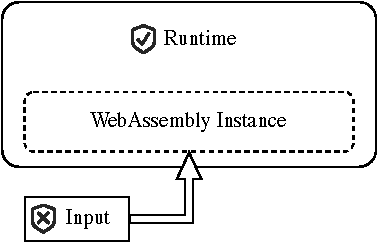
\includegraphics{figures/build/wasm-internal-mem-safety}
        \caption{Internal Memory Safety}
        \label{fig:internal-mem-safety}
    \end{subfigure}
    \hfill
    \begin{subfigure}[T]{0.45\textwidth}
        \centering
        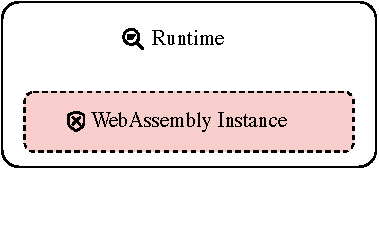
\includegraphics{figures/build/wasm-external-mem-safety}
        \caption{External Memory Safety}
        \label{fig:external-mem-safety}
    \end{subfigure}
    \caption{Threat model for internal and external memory safety}
    \label{fig:threat-model}
\end{figure}

\begin{description}
    \item[Internal Memory Safety:] Ensures memory safety within the boundaries of a sandbox.
    Our point of view is that from within a WebAssembly instance, we trust the runtime (and the host we are running on), but we do not trust external input.
    See \cref{fig:internal-mem-safety}
    \item[External Memory Safety:] Maintains the memory safety of the sandbox itself against potentially malicious programs.
    Our point of view is from the runtime; we trust the platform we are running on but not the WebAssembly programs we are executing.
    See \cref{fig:external-mem-safety}
\end{description}

\subsection{Internal Memory Safety}
\label{subsec:internal-memory-safety}
For internal memory safety, the program within the sandbox and its runtime, including its compiler, are considered trusted and assumed to be bug-free.
Untrusted input (e.g., network data, file reads) originates from outside the sandbox and may be controlled by an attacker.
This model mirrors the threat environment of a standard non-\ac{WASM} program.
Potential threats include:

\begin{itemize}
    \item \textbf{Buffer overflows} Attempts to access memory beyond allocated buffer boundaries.
    \item \textbf{Use-after-free} Attempts to access deallocated memory.
\end{itemize}

As discussed in \cref{sec:wasm}, WebAssembly's design inherently mitigates some threats common in non-\ac{WASM} environments, so we will not consider the following vectors:

\begin{itemize}
    \item \textbf{Return-oriented attacks} {\ac{WASM}'s} structured control flow constructs prevent arbitrary code execution through stack manipulation.
    \item \textbf{Calling unknown function pointers} Function tables enforce a strict mechanism for function calls, ensuring the integrity of call targets.
\end{itemize}

\subsection{External Memory Safety}
\label{subsec:external-memory-safety}

For external memory safety, we focus on the security of the sandbox.
Threats originate from running untrusted programs, which may be buggy or adversarial.

\begin{itemize}
    \item \textbf{Sandbox escapes}: Attempts to break out of the sandbox's restrictions and access host resources.
    \item \textbf{Side-channel attacks}: Exploiting timing differences or resource usage patterns to infer sensitive information.
\end{itemize}

We assume that the operating system and underlying target architecture are free of bugs that malicious targets might exploit.
This does not include assumptions about potential spectre-like~\cite{kocher2020spectre} attacks.
The compiler needs to ensure that bounds checks are guarded against side-channel attacks.

Additionally, we do not consider exploits of the program running in the sandbox as vulnerabilities.
Regarding the runtime, as long as exploits are contained within the sandbox, the security objectives have been met.

\section{Overview}
\label{sec:overview}

\begin{figure*}[t]
    \centering
    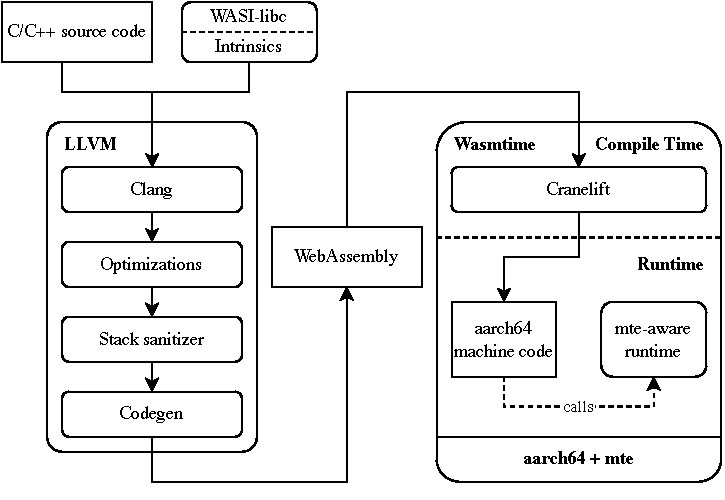
\includegraphics{figures/build/overview}
    \caption{Overview of the adapted workflow}
    \label{fig:overview}
\end{figure*}

Figure~\ref{fig:overview} presents an overview of our prototype.

At build time, the unmodified C/C++ sources and a modified version of libc are compiled using LLVM~\cite{lattner2004llvm}.
After optimizations, a stack sanitizer analyzes all functions and inserts instrumentation as necessary.
LLVM's backend then generates WebAssembly binaries that can be deployed and executed on a wide variety of devices.

\section{WebAssembly Extension}
\label{sec:wasm-extension}

We designed an extension to WebAssembly that provides primitives to the modified standard library and the stack sanitizer to guarantee memory safety for selected allocations.
Our extension builds on wasm64, the 64\,bit variant of WebAssembly.
We chose wasm64, as wasm64 uses a 64\,bit integer index type, with 48 of those bits used to index memory.
This allows for the utilization of 16 bits of metadata per pointer.

For our extension, we introduce the notion of abstract segments and tagged pointers.
We introduce three new instructions that allow the creation of abstract segments and tagged pointers from raw pointers.
These pointers carry provenance and can only access the segment they were created with.
Conversely, segments can only be accessed by the tagged pointer created with them rather than with raw indices without provenance.
The instructions are type-checked according to \cref{fig:typing-rules}.

\begin{equation*}
    \text{(new instructions) } e \Coloneqq \textbf{segment.new} \mid \textbf{segment.set\_tag} \mid \textbf{segment.free}
\end{equation*}


\begin{figure}[t]
    \begin{prooftree}
        \AxiomC{$C_{\text{memory}} = n$}
        \AxiomC{$2^a=16$}
        \BinaryInfC{$C \vdash \textbf{segment.new}\ a\ o : \text{i64}\ \text{i64} \rightarrow \text{i64}$}
    \end{prooftree}
    \begin{prooftree}
        \AxiomC{$C_{\text{memory}} = n$}
        \AxiomC{$2^a=16$}
        \BinaryInfC{$C \vdash \textbf{segment.set\_tag}\ a\ o : \text{i64}\ \text{i64}\ \text{i64} \rightarrow \epsilon$}
    \end{prooftree}
    \begin{prooftree}
        \AxiomC{$C_{\text{memory}} = n$}
        \AxiomC{$2^a=16$}
        \BinaryInfC{$C \vdash \textbf{segment.free}\ a\ o : \text{i64}\ \text{i64} \rightarrow \epsilon$}
    \end{prooftree}
    \caption{Typing rules}
    \label{fig:typing-rules}
\end{figure}

\paragraph{}
In the following paragraph, we will describe the new instructions in detail.

\begin{description}
    \item[\texttt{segment.new}] Create a new, zeroed memory segment.
    This instruction takes two parameters: a memory index and a size.
    The instruction generates a new tag, assigns it to the piece of memory, and returns a tagged pointer that can be used to access the segment.
    \item[\texttt{segment.set\_tag}] Takes a memory index, a length, and a tagged pointer and applies the tag from the tagged pointer to the memory segment located at the index with the passed length.
    This can be used to move ownership from one segment to another or to merge segments.
    \item[\texttt{segment.free}] Invalidates a segment by reassigning a new, implementation-defined tag.
    This instruction takes two parameters: a memory index and a length.
    After this instruction, the tagged pointer being used to access the segment is no longer valid, and accessing the segment through it will result in a trap.
\end{description}

We also modify the semantics of existing load and store instructions.
They still take an integer as an index, but we introduce provenance to integers, which we can track at runtime using the unused 16 upper bits in pointers.
If a segment is accessed, the runtime will check that the tagged pointer is allowed to access the segment, i.e., the metadata matches the metadata created by the \texttt{segment.new} instruction.
If this is not the case, the runtime throws a trap

At startup, the linear memory consists of a single segment that can be accessed using untagged indices, allowing unmodified code to run under our new semantics without modifications.
This design choice also allows the gradual integration of safety primitives into specific parts of WebAssembly applications where enhanced security is required.
For instance, it enables the introduction of a hardened malloc implementation, which prevents spatial and temporal safety bugs for heap-allocated memory.
Additionally, we can analyze stack allocations to only harden those accessed using untrusted indices or escape our analysis, e.g., by taking their address and passing it to another function.
Safe slots, such as spill slots, do not have to be instrumented, improving performance.

\paragraph{Alignment}
All segments are aligned to 16 bytes, corresponding to the alignment of MTE (see \cref{subsec:mte}).
This is an implementation choice that may be changed once we support additional implementations.
More detail can be found in \cref{sec:future-work}.

\subsection{Example}
\label{subsec:example}

We will demonstrate our \ac{WASM} extension using the following C snippet, which allocates 64 bytes on the stack.
\begin{lstlisting}[frame=h,style=customc,
    label={lst:wasm-example-c}]
void foo() {
    char buf[64];
    // ...
    return;
}
\end{lstlisting}

This requires the compiler to instrument the stack allocation, create a new segment, and free the segment before returning to the caller, i.e., giving ownership of the stack slot back to the stack frame.
We show the resulting code below.

\begin{lstlisting}[frame=h,style=customwasm,
    label={lst:wasm-example}]
;; Allocate space on the stack
global.get $__stack_pointer
i64.const 64
i64.sub
global.tee $__stack_pointer

;; create a segment
i64.const 64
segment.new
local.set $buf

;; ...

;; retag with stack pointer tag
local.get $buf
global.get $__stack_pointer
i64.const 64
segment.set_tag

;; reset stack pointer
global.get $__stack_pointer
i64.const 64
i64.sub
global.set $__stack_pointer
\end{lstlisting}

The compiler allocates the slot for \texttt{buf} on the stack, decrementing the global \texttt{\$\_\_stack\_pointer} acting as the stack pointer.
Then, a new segment of size 64 is created, and the tagged pointer to it is stored in the local \lstinline[style=customwasm]{$buf}.
Before returning, the segment is retagged using the stack pointers tag, i.e., restoring the previous tag and allowing access through the stack pointer.
Then, the stack pointer is reset, freeing the stack frame.

\subsection{Heap Safety}
\label{subsec:heap-safety}

The memory allocator needs to be aware of segments to provide heap safety.
When allocating memory, it aligns the requested size to 16 bytes, creates a segment, and returns the corresponding tagged pointer.
This prevents overflows from corrupting allocator metadata or other memory segments.

\subsection{Stack Safety}
\label{subsec:stack-safety}

For stack safety, we create segments from stack slots when entering a function.
Before returning, all stack slots are untagged and reassigned to the stack frame.
This allows other functions to use the memory and prevents stack slots from being accessed after returning from a function.

However, only some stack slots need to be turned into segments, e.g., spill slots, stack slots that do not escape, or stack slots that are only indexed into using an index we can statically check to be in bounds.
Creating segments for these would create excessive runtime and memory overhead, as each stack slot would need to be aligned to 16 bytes and processed when entering and returning from a function.

To address this, we designed an algorithm that identifies safe memory regions within the stack that do not require protection, thus avoiding creating segments for the slots mentioned above.
Below, we present a simplified version of our algorithm.
We iterate over all stack allocations and check if the allocation (a) escapes the function or (b) is indexed into using an unsafe \ac{GEP} instruction.

\begin{algorithmic}
    \State $allocsToInstrument \gets \emptyset$
    \For{$alloc \in allocations$}
        \If{escapes($alloc$)}
            \State $allocsToInstrument \gets allocsToInstrument \cup \{\,alloc\,\}$
        \ElsIf{isUsedByUnsafeGEP($alloc$)}
        \State $allocsToInstrument \gets allocsToInstrument \cup \{\,alloc\,\}$
        \EndIf
    \EndFor

    \For{$alloc \in allocsToInstrument$}
        \State insertTaggingCode($alloc$)
        \State insertUntaggingCode($alloc$)
    \EndFor
\end{algorithmic}

\subsection{Example}
\label{subsec:example2}

We demonstrate the algorithm using the following function.

\begin{lstlisting}[frame=h,style=customc,
    label={lst:stack-safety}]
char foo(int index) {
  int i = 0; // safe
  int bytes_read = 0; // unsafe
  char buf[32]; // unsafe
  read_input(buf, &bytes_read);
  return buf[index];
}

char *bar() {
    char buf[32]; // unsafe
    return buf;
}
\end{lstlisting}

In the code example above, \texttt{i} is safe, as its address is not used in a potentially unsafe address computation and does not escape.
The variables \texttt{bytes\_read} and \texttt{buf} are deemed unsafe as their address escapes.
Additionally, \texttt{buf} is accessed using an untrusted index.

In function \texttt{bar}, \texttt{buf} also needs to be instrumented as it escapes: the pointer to it is returned to the caller.
Any attempt to dereference the value returned by \texttt{bar} is undefined behavior and will be caught by our instrumentation, preventing difficult-to-debug bugs or potential vulnerabilities.

\noindent
This algorithm effectively balances the need for stack safety with performance and memory efficiency constraints.
